\chapter{Implementação: InvestiGator}
\label{cap:sistema}

Este capítulo descreve a realização do sistema: a sua arquitetura, a forma como cada método do
Capítulo~\ref{cap:metodologia} é concretizado, a política que decide o que é comunicado ao
utilizador, a construção da mensagem entregue, e o ciclo de vida do componente aprendido.

O Capítulo~\ref{cap:metodologia} apresentou quatro métodos de forma isolada. A sua composição num sistema em funcionamento introduz problemas que nenhum deles apresenta
isoladamente: a indisponibilidade das fontes, o volume de candidatos por ciclo, a coerência entre
os valores calculados e o texto apresentado, e a degradação silenciosa dos componentes ao longo do
tempo. A descrição que se segue organiza-se em
torno desses problemas.

O sistema desenvolvido designa-se por InvestiGator e encontra-se em funcionamento contínuo,
entregando alertas a um canal de mensagens e disponibilizando o registo das suas decisões numa
aplicação web. Os valores apresentados neste capítulo foram lidos do registo do sistema em
operação, e as datas em que cada medição foi efetuada são indicadas junto de cada uma.

\section{Arquitetura do sistema}
\label{sec:sis_arquitetura}

A arquitetura do InvestiGator foi definida de acordo com os seguintes requisitos, relativos a
custo, modularidade, verificabilidade e resiliência:

\begin{itemize}
  \item operar exclusivamente sobre fontes de dados gratuitas, sem subscrições nem custos por
        pedido;
  \item isolar cada método num componente com responsabilidade única, substituível sem alteração
        dos restantes;
  \item garantir que qualquer valor apresentado ao utilizador tem origem no componente que o
        calculou, e não numa segunda derivação independente;
  \item tolerar a indisponibilidade de qualquer fonte externa sem interrupção do serviço;
  \item registar cada decisão tomada, incluindo as decisões de não comunicar.
\end{itemize}

O sistema organiza-se em cinco componentes, representados na Figura~\ref{fig:sis_arquitetura}:
deteção, recuperação, triagem, explicação e entrega. A decomposição do movimento constitui um
sexto componente, ativado apenas no percurso iniciado por movimento de preço, uma vez que a
repartição incide sobre o retorno do dia e não existe objeto a repartir quando o acontecimento
que desencadeia a avaliação é uma notícia.

\begin{figure}[ht]
\centering
\begin{tikzpicture}[
  font=\small, >={Stealth[length=2.4mm]},
  cx/.style={draw, rounded corners, align=center, text width=2.6cm, minimum height=1.5cm,
             inner sep=4pt},
  fonte/.style={cx, fill=black!10},
  proc/.style={cx, fill=black!3},
  saida/.style={cx, fill=black!16},
]
  \node[fonte] (p) {\textbf{Preços}\\ \footnotesize cadeia de quatro\\ \footnotesize alternativas};
  \node[fonte, below=6mm of p] (n) {\textbf{Notícias}\\ \footnotesize três interfaces\\ \footnotesize gratuitas};
  \node[fonte, below=6mm of n] (h) {\textbf{Base de casos}\\ \footnotesize precedentes com\\ \footnotesize impacto medido};

  \node[proc, right=0.8cm of p] (det) {\textbf{Deteção}\\ \footnotesize $z$-score};
  \node[proc, right=0.8cm of n] (rec) {\textbf{Recuperação}\\ \footnotesize vizinhos semânticos};
  \node[proc, right=0.8cm of h] (tri) {\textbf{Triagem}\\ \footnotesize probabilidade calibrada};
  \node[proc, dashed, below=6mm of tri] (dec)
    {\textbf{Decomposição}\\ \footnotesize mercado, setor,\\ \footnotesize empresa};

  \node[proc, right=0.9cm of rec, text width=2.8cm] (exp)
    {\textbf{Explicação}\\ \footnotesize composição a partir\\ \footnotesize dos objetos\\ \footnotesize calculados};

  \node[saida, right=0.8cm of exp, yshift=9mm] (tg) {\textbf{Canal de mensagens}};
  \node[saida, right=0.8cm of exp, yshift=-9mm] (web) {\textbf{Aplicação web}\\ \footnotesize registo de decisões};

  \draw[->] (p) -- (det);
  \draw[->] (n) -- (rec);
  \draw[->] (h) -- (tri);
  \draw[->] (h.east) -- ++(0.35,0) |- (rec.west);
  \draw[->] (det.east) -- ++(0.4,0) |- (exp.west);
  \draw[->] (rec) -- (exp);
  \draw[->] (tri.east) -- ++(0.4,0) |- (exp.west);
  \draw[->, dashed] (p.south west) -- ++(-0.35,0) |- (dec.west);
  \draw[->, dashed] (dec.east) -- ++(0.55,0) |- (exp.west);
  \draw[->] (exp.east) -- ++(0.35,0) |- (tg.west);
  \draw[->] (exp.east) -- ++(0.35,0) |- (web.west);
\end{tikzpicture}
\caption[Arquitetura do InvestiGator]{Componentes do sistema e respetivas ligações. À esquerda, as
fontes de dados; ao centro, os métodos do Capítulo~\ref{cap:metodologia} e o componente que compõe
o texto; à direita, os dois canais de entrega. A decomposição encontra-se a tracejado por ser o
único componente que não intervém em todas as avaliações.}
\label{fig:sis_arquitetura}
\end{figure}

Uma regra de construção atravessa a totalidade da implementação: o texto entregue ao utilizador é
composto a partir dos objetos que os componentes produziram, e não redigido de forma independente.
Quando o detetor calcula um valor de $z$ igual a $+7{,}61$, é esse valor que a mensagem apresenta.
A alternativa, que consistiria em manter um local onde o texto é escrito e outro onde a quantidade
é calculada, admite divergência entre os dois sem que essa divergência seja observável. A
restrição elimina essa possibilidade por construção.

\subsection{Comunicação entre componentes}

Os componentes comunicam por passagem direta de objetos dentro de um processo único, e não por
protocolo de rede. A decisão decorre do perfil de utilização: o sistema serve uma lista reduzida
de empresas, com um ciclo de avaliação de sessenta segundos, e o volume não justifica o custo de
coordenação de uma arquitetura distribuída. A separação entre componentes é assegurada por
interfaces explícitas, o que preserva a substituibilidade sem introduzir latência de comunicação.

Duas exceções operam sobre fronteiras de processo. A entrega utiliza a interface de robô do canal
de mensagens, por pedido HTTP. A aplicação web que expõe o registo de decisões corre como processo
separado e lê o mesmo repositório de dados, sem escrever nele. Esta segunda separação garante que
a consulta do registo não interfere com o ciclo de avaliação.

\section{Aquisição de dados}
\label{sec:sis_dados}

A restrição de custo nulo determina as decisões de aquisição. Um investidor particular que
considere elevados os custos de corretagem não subscreve um terminal de informação financeira, e a
utilidade do sistema para o destinatário definido no Capítulo~\ref{cap:introducao} depende de o
sistema operar sem esse custo. As fontes gratuitas apresentam, contudo, três limitações
sistemáticas: bloqueiam o acesso por excesso de pedidos, respondem com erro sem aviso, e publicam
com atraso. As decisões descritas nesta secção respondem a essas limitações.

\subsection{Preços}

Os preços são obtidos através de uma cadeia de quatro alternativas, consultadas por ordem fixa,
adotando-se a primeira que responde com dados válidos. O identificador da fonte que serviu cada
valor é registado juntamente com o valor, uma vez que a proveniência de uma quantidade integra a
sua explicação.

A ordem da cadeia não é arbitrária nem definitiva. Uma das fontes foi despromovida na sequência da
observação do conteúdo que devolvia, e uma candidata adicional foi rejeitada por responder com
verificação anti-robô, o que a torna inutilizável em operação automática. Estas duas decisões
resultaram de medição e não de preferência declarada.

A redundância da cadeia tem uma consequência que ultrapassa a disponibilidade. Sem ela, um dia em
que a fonte única bloqueia o acesso é indistinguível de um dia em que o mercado não abriu, e o
sistema não dispõe de forma de separar as duas situações.

\subsection{Notícias}
\label{sec:sis_fontes}

As notícias são obtidas por empresa, a partir de três interfaces gratuitas. O material recebido
inclui um volume elevado de conteúdo não aproveitável: listas automáticas de maiores variações do
dia, textos que mencionam a empresa apenas de passagem, e comunicados de escritórios de advocacia.
Um filtro de relevância, aplicado à entrada, exige que o título nomeie explicitamente a empresa e
rejeita os padrões conhecidos de texto gerado automaticamente.

A utilização de três fontes em vez de uma foi avaliada por medição, sobre doze empresas e três
dias. O critério adotado não é o número de títulos devolvidos por cada fonte, mas o número de
títulos que sobrevive ao filtro de relevância, dado que o material rejeitado à entrada não chega a
existir para o sistema. A Tabela~\ref{tab:sis_fontes} apresenta o resultado.

\begin{table}[!htbp]
\caption[Caracterização das três fontes de notícias]{Material entregue por cada fonte gratuita
após aplicação do filtro de relevância. A coluna \emph{exclusivos} indica os títulos que uma fonte
traz e nenhuma das outras traz. Esse valor constitui um limite superior, uma vez que a comparação
entre títulos é efetuada por correspondência textual após normalização, e duas fontes que
descrevam o mesmo acontecimento por outras palavras produzem dois títulos contabilizados como
distintos.}
\label{tab:sis_fontes}
\centering
\small
\begin{tabular}{L{0.20\textwidth} C{0.12\textwidth} C{0.11\textwidth} C{0.13\textwidth}
                C{0.12\textwidth} C{0.13\textwidth}}
\toprule
\tabhead{Fonte} & \tabhead{Relevantes} & \tabhead{Precisão} & \tabhead{Frescura} &
\tabhead{Cobertura} & \tabhead{Exclusivos} \\
\midrule
Finnhub & $432$ & $\mathbf{35\%}$ & $15{,}8$ h & $\mathbf{12/12}$ & $401$ \\
Alpha Vantage & $141$ & $24\%$ & $\mathbf{9{,}3}$ \textbf{h} & $\mathbf{12/12}$ & $119$ \\
Polygon & $429$ & $27\%$ & $52{,}6$ h & $8/12$ & $\mathbf{418}$ \\
\bottomrule
\end{tabular}
\end{table}

As três fontes apresentam perfis complementares, e é essa complementaridade, e não o volume
agregado, que justifica a sua utilização conjunta. O Finnhub apresenta a maior precisão de
etiquetagem e cobre a totalidade das empresas. A Alpha Vantage apresenta a menor mediana de idade
das notícias, com $9{,}3$ horas contra $15{,}8$, o que a torna a fonte relevante para a redução do
atraso dos alertas. O Polygon contribui com o maior número de títulos exclusivos, com uma mediana
de idade de $52{,}6$ horas, o que o torna adequado à alimentação da base de casos e inadequado ao
alerta em tempo útil. É essa a utilização que lhe está atribuída.

O conjunto das três fontes produz $970$ títulos relevantes distintos, contra os $432$ obtidos
apenas com o Finnhub. O ganho concentra-se nas empresas com menor cobertura individual, que
correspondem precisamente aos casos em que o sistema anteriormente não dispunha de material para
comentar.

A agregação não garante, contudo, redução da latência em geral. As três fontes publicam com
atrasos próprios, e o ganho num caso concreto depende de qual delas observou o acontecimento em
primeiro lugar. A mediana de frescura melhora, e essa melhoria encontra-se medida; a afirmação de
que os alertas passam a chegar mais cedo exigiria nova medição da latência de extremo a extremo
sobre um período alargado, que não foi realizada.

\subsection{Base histórica e base implantada}

A recuperação de precedentes requer um corpo de casos passados com desfecho conhecido. O sistema
utiliza dois conjuntos distintos, com finalidades distintas, e a sua separação é relevante para a
leitura dos resultados do Capítulo~\ref{cap:avaliacao}.

O primeiro é o \gls{FNSPID} \autocite{dong2024fnspid}, um conjunto público de notícias financeiras
alinhado com os preços correspondentes. Do alinhamento descrito na Secção~\ref{sec:met_dados}
resultam $79\,753$ exemplos entre 2018 e 2023, cada um com o movimento de preço subsequente. É
sobre este conjunto que os métodos são avaliados.

O segundo é a base de casos que o sistema implantado consulta, e resulta da fusão de duas origens
que importa não confundir. A primeira é uma reconstrução de um ano de história, obtida executando os
componentes de recolha e de maturação sobre o passado, com $38\,214$ casos; a separação face ao
registo do sistema em funcionamento é deliberada, uma vez que um caso reproduzido não é um caso
observado. A segunda é a base viva, alimentada pela varredura, com $11\,445$ casos. A recuperação
percorre as duas em conjunto. Os vetores são armazenados como matriz de precisão simples mapeada em disco. O
formato não é indiferente: as mesmas representações em estruturas nativas da linguagem excediam a
memória disponível no contentor de execução, e a alteração de formato foi a condição que tornou a
sua utilização possível.

\section{Percurso de um acontecimento}
\label{sec:sis_percurso}

O sistema admite dois percursos distintos, consoante o acontecimento que desencadeia a avaliação
seja uma notícia ou um movimento de preço. Os dois convergem no componente de explicação e
utilizam a mesma política de decisão, descrita na Secção~\ref{sec:sis_politica}.

\subsection{Percurso iniciado por notícia}

O percurso iniciado por notícia compreende nove etapas, representadas na
Figura~\ref{fig:sis_caminho}. Quatro dessas etapas são pontos de decisão em que a candidata pode
ser descartada, situação em que o sistema não comunica.

\begin{figure}[ht]
\centering
\begin{tikzpicture}[
  font=\footnotesize, >={Stealth[length=2mm]},
  et/.style={draw, rounded corners, align=center, text width=2.15cm, minimum height=1.15cm,
             fill=black!3},
  porta/.style={et, dashed, fill=black!12},
  n/.style={font=\bfseries\footnotesize, text=black!45},
]
  \node[et] (a) {recolher\\ notícias};
  \node[porta, right=4mm of a] (b) {nomeia a\\ empresa?};
  \node[porta, right=4mm of b] (c) {é recente?};
  \node[et, right=4mm of c] (d) {recuperar\\ precedentes};
  \node[porta, below=7mm of d] (e) {evidência\\ suficiente?};
  \node[porta, left=4mm of e] (f) {triagem\\ acima do\\ piso?};
  \node[porta, left=4mm of f] (g) {já comunicado\\ hoje?};
  \node[et, left=4mm of g] (h) {compor a\\ explicação};
  \node[et, below=7mm of h, fill=black!16] (i) {entregar e\\ registar};

  \foreach \x/\i in {a/1, b/2, c/3, d/4} { \node[n, above=0.5mm of \x] {\i}; }
  \foreach \x/\i in {e/5, f/6, g/7, h/8} { \node[n, above=0.5mm of \x] {\i}; }
  \node[n, above=0.5mm of i] {9};

  \draw[->] (a) -- (b); \draw[->] (b) -- (c); \draw[->] (c) -- (d);
  \draw[->] (d) -- (e); \draw[->] (e) -- (f); \draw[->] (f) -- (g); \draw[->] (g) -- (h);
  \draw[->] (h) -- (i);
\end{tikzpicture}
\caption[Etapas do percurso iniciado por notícia]{As nove etapas do percurso. As caixas a
tracejado correspondem a pontos de decisão em que a candidata pode ser descartada. A
Secção~\ref{sec:sis_politica} quantifica a proporção de candidatas eliminada em cada um.}
\label{fig:sis_caminho}
\end{figure}

O funcionamento do percurso é ilustrado por um alerta entregue a 12 de julho de 2026, relativo à
Meta, com o título \emph{``Mark Zuckerberg Said Meta's AI Bets `Haven't Come to Fruition Yet' as
Shares Fell 5\%''}. O título nomeia a empresa e não corresponde a nenhum dos padrões de texto automático. A data
situa-se dentro do intervalo de dois dias exigido. Os três precedentes mais próximos são Microsoft
de 2023-11-07, com semelhança $0{,}46$, Nvidia de 2023-08-02, com $0{,}51$, e Nvidia de
2023-09-21, com $0{,}46$; a melhor delas fica acima do limiar de $0{,}45$. O modelo de triagem
atribui uma probabilidade de $54\%$. E o alerta é o primeiro relativo à empresa nesse dia. A mensagem é então composta e registada.

Os precedentes recuperados neste caso pertencem a empresas distintas daquela sobre a qual o alerta
incide, e são apresentados na mesma. A opção é deliberada e decorre da formulação da terceira
questão de investigação: a comparabilidade é estabelecida pelo tema da notícia e não pela
identidade da empresa. Notícias relativas a investimento em inteligência artificial em empresas
tecnológicas de grande dimensão constituem casos comparáveis entre si.

Os desfechos dos três precedentes são divergentes, com movimentos de $+2{,}70\%$, $-3{,}87\%$ e
$+5{,}05\%$. O sistema apresenta os três individualmente, e não a sua média, precisamente por essa
razão. A média oculta a informação mais relevante do conjunto, que é a inexistência de um desfecho
comum a casos semelhantes.

\subsection{Percurso iniciado por movimento de preço}

O segundo percurso é substancialmente mais curto. O $z$-score é calculado por dois caminhos. Após o
fecho de cada sessão, o sistema avalia o retorno do dia fechado de cada empresa da lista vigiada
contra a norma dos vinte dias anteriores, conforme descrito na Secção~\ref{sec:met_detecao}. Durante
a sessão, avalia o retorno em curso, obtido da cotação corrente contra o fecho anterior, contra a
mesma norma diária, formada nesse caso pelos vinte dias completos mais recentes, uma vez que o dia
em curso ainda não pertence à série. O segundo caminho antecipa a deteção sem alterar a definição de
normalidade, e é o que permite comunicar um movimento enquanto a sessão decorre; é também o que não
depende da fonte de séries históricas, cuja barra do dia pode chegar com atraso. Em qualquer dos
caminhos, a ultrapassagem do limiar constitui condição suficiente para avaliação.

É neste percurso, e apenas neste, que intervém a decomposição do movimento. Ao alerta é acrescentada
uma linha com a repartição calculada segundo a Secção~\ref{sec:met_decomposicao}, com a forma
\emph{``NFLX $-2{,}11\%$ hoje $=$ $-0{,}08\%$ mercado $\cdot$ $-0{,}32\%$ setor $\cdot$
$-1{,}71\%$ da própria empresa''}, seguida de uma frase que nomeia em linguagem corrente a parcela
dominante. Quando a estimação da sensibilidade ao mercado não é possível, a linha é apresentada na
mesma, declarando que foi assumida sensibilidade unitária e que a repartição tem carácter
indicativo.

Duas capacidades foram acrescentadas ao percurso após a entrada do sistema em funcionamento, ambas
por observação do comportamento em operação. A primeira consiste na atribuição de níveis de
severidade: um valor de $z$ de $1{,}6$ e um valor de $3{,}2$ passaram a ser descritos por termos
distintos, em lugar de gerarem a mesma formulação. A segunda consiste na comparação com as
restantes empresas do mesmo setor na mesma sessão, dado que um alerta que reporta uma descida sem
indicar que o setor inteiro desceu transmite informação incompleta.

A segunda correção resultou da leitura dos trinta primeiros alertas entregues. Em nove deles o
texto era internamente contraditório: uma linha indicava que o movimento parecia comum ao setor, e
a repartição apresentada duas linhas abaixo atribuía a maior parcela à empresa. As duas linhas
estavam corretas isoladamente, e a contradição resultava de a comparação com os pares considerar
apenas a direção do movimento das empresas vizinhas, e não a sua magnitude. A comparação passou a
considerar ambas.

\section{Política de decisão}
\label{sec:sis_politica}

A comunicação de todas as candidatas avaliadas é equivalente à ausência de comunicação. Um canal
que entregue quinze mensagens diárias deixa de ser lido, e o sistema perde a utilidade que
justifica a sua existência. Os pontos de decisão da Figura~\ref{fig:sis_caminho} respondem a esta
restrição.

\subsection{Seletividade observada}

O efeito conjunto dos pontos de decisão é considerável. Sobre as notícias datadas entre 4 e 13 de julho de
2026, das $944$ notícias relevantes que entraram no sistema resultaram $42$ alertas, o que
corresponde a uma razão aproximada de um para vinte e dois. O valor é um limite superior da
seletividade da política atual, uma vez que o limite de duas mensagens por empresa entrou em vigor a
11 de julho, a meio da janela observada. A Figura~\ref{fig:sis_seletividade} apresenta a
distribuição por empresa.

\begin{figure}[ht]
\centering
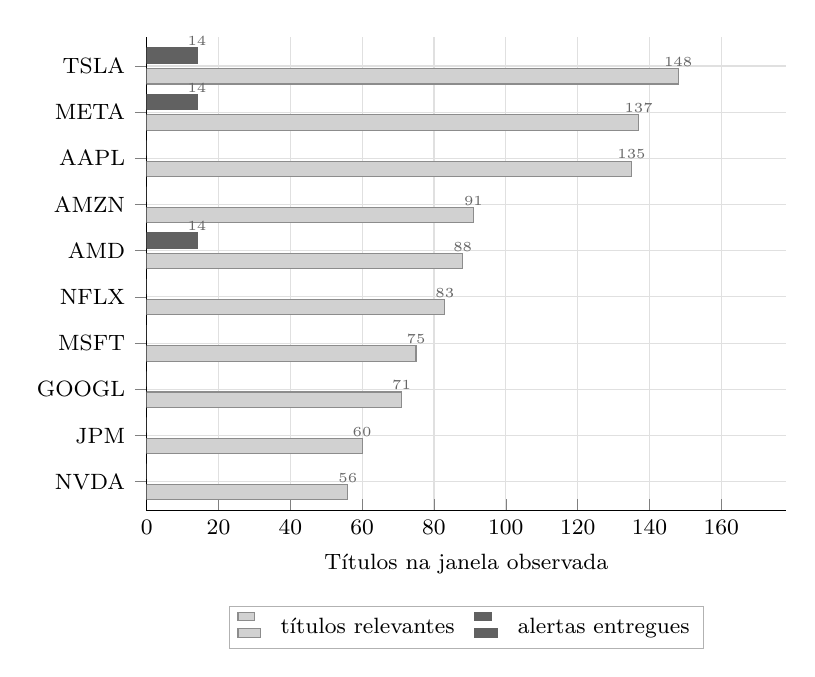
\begin{tikzpicture}
\begin{axis}[
  xbar, width=0.80\textwidth, height=7.6cm,
  xmin=0, xmax=178,
  bar width=5.5pt,
  enlarge y limits=0.07,
  symbolic y coords={NVDA,JPM,GOOGL,MSFT,NFLX,AMD,AMZN,AAPL,META,TSLA},
  ytick={NVDA,JPM,GOOGL,MSFT,NFLX,AMD,AMZN,AAPL,META,TSLA},
  xlabel={Títulos na janela observada},
  tick label style={font=\footnotesize},
  label style={font=\footnotesize},
  legend style={font=\footnotesize, at={(0.5,-0.20)}, anchor=north, legend columns=2,
                draw=black!30, column sep=1.2ex},
  point meta=explicit symbolic,
  nodes near coords, nodes near coords style={font=\tiny, black!60},
  grid=major, grid style={black!12},
  axis lines*=left,
]
\addplot[fill=black!18, draw=black!45] coordinates {
  (56,NVDA) [56] (60,JPM) [60] (71,GOOGL) [71] (75,MSFT) [75] (83,NFLX) [83]
  (88,AMD) [88] (91,AMZN) [91] (135,AAPL) [135] (137,META) [137] (148,TSLA) [148]};
\addplot[fill=black!62, draw=black!62] coordinates {
  (0,NVDA) [] (0,JPM) [] (0,GOOGL) [] (0,MSFT) [] (0,NFLX) []
  (14,AMD) [14] (0,AMZN) [] (0,AAPL) [] (14,META) [14] (14,TSLA) [14]};
\legend{títulos relevantes, alertas entregues}
\end{axis}
\end{tikzpicture}
\caption[Seletividade do sistema por empresa]{Títulos relevantes captados e alertas efetivamente
entregues, por empresa, na janela observada. O total é de $944$ títulos e $42$ alertas. A
concentração dos alertas em três empresas não resulta de qualquer regra que privilegie essas
empresas: decorre da interação entre o limiar de semelhança e a composição da base de casos, cuja
cobertura por empresa é desigual. A Secção~\ref{sec:av_producao} confirma-o sobre uma amostra
muito maior.}
\label{fig:sis_seletividade}
\end{figure}


O comportamento num único dia permite localizar a eliminação de candidatas. A
Figura~\ref{fig:sis_funil} distribui as $5\,060$ avaliações registadas a 15 de agosto de 2026 pelo
ponto de decisão em que cada uma terminou. O registo lido corresponde a parte do dia e não ao dia
completo, pelo que os valores devem ser lidos como proporções.

\begin{figure}[ht]
\centering
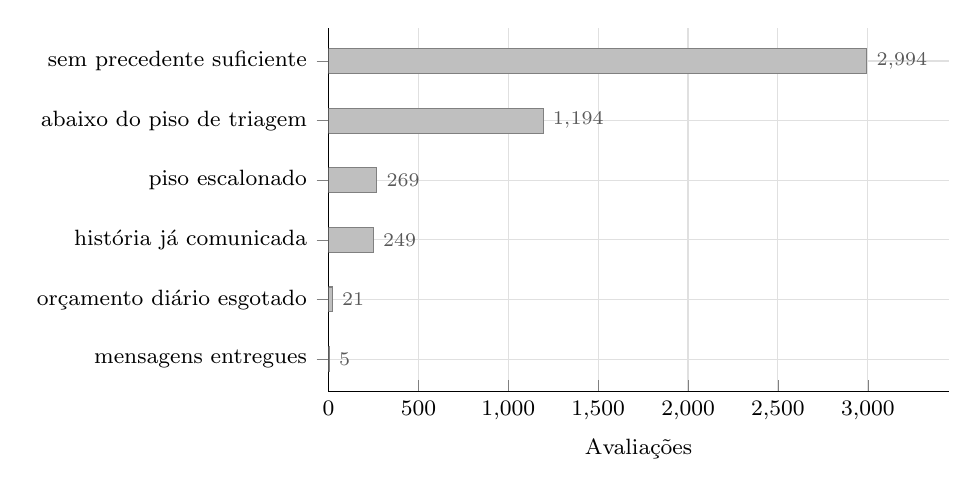
\begin{tikzpicture}[font=\footnotesize]
\begin{axis}[
  xbar, width=0.78\textwidth, height=6.2cm,
  xmin=0, xmax=3450,
  bar width=9pt,
  enlarge y limits=0.11,
  symbolic y coords={entregues,orcamento,repetida,escada,triagem,precedente},
  ytick=data,
  yticklabels={{mensagens entregues},{orçamento diário esgotado},{história já comunicada},
               {piso escalonado},{abaixo do piso de triagem},{sem precedente suficiente}},
  xlabel={Avaliações},
  tick label style={font=\footnotesize},
  label style={font=\footnotesize},
  nodes near coords, nodes near coords style={font=\scriptsize, black!65},
  grid=major, grid style={black!12},
  axis lines*=left,
]
\addplot[fill=black!25, draw=black!50] coordinates {
  (5,entregues) (21,orcamento) (249,repetida) (269,escada) (1194,triagem) (2994,precedente)};
\end{axis}
\end{tikzpicture}
\caption[Distribuição das avaliações de um dia pelos pontos de decisão]{As $5\,060$ avaliações
registadas a 15 de agosto de 2026, distribuídas pelo ponto em que cada uma terminou. As $333$
avaliações que atravessaram todos os pontos de decisão não figuram no gráfico, pela razão
apresentada no texto. O orçamento diário de cinco mensagens foi integralmente utilizado. A data é
também a do dia em que o piso de triagem deixou de exercer veto e passou a ordenar, pelo que a barra
de $1\,194$ avaliações eliminadas nesse ponto pertence à configuração anterior à descrita na
Tabela~\ref{tab:sis_portas}; nos dias seguintes esse ponto deixa de eliminar candidatas.}
\label{fig:sis_funil}
\end{figure}

A leitura destes valores expõe um defeito de instrumentação. As $333$ avaliações que atravessaram
todos os pontos de decisão não correspondem a $333$ candidatas distintas aprovadas para entrega. O
sistema reavalia os mesmos títulos em cada ciclo de sessenta segundos, e um título já entregue
nesse dia voltava a atravessar todos os pontos de decisão em cada ciclo. A entrega era impedida no
final, por uma verificação de duplicação que, ao contrário de todas as restantes, não estava
registada como etapa.

A consequência é relevante para a finalidade do registo. A vista construída para tornar as
decisões do sistema inspecionáveis indicava $333$ aprovações num dia em que foram entregues cinco
mensagens. A verificação de duplicação passou a constituir uma etapa com identificação própria,
como as restantes, e existe um teste automático que falha caso volte a ser omitida. Os valores da
figura são anteriores a essa correção.

\subsection{Limiares e sua proveniência}

Cada ponto de decisão utiliza uma constante, e a origem dessas constantes é heterogénea. A
Tabela~\ref{tab:sis_portas} distingue os valores derivados de uma análise dos valores escolhidos,
distinção que é pertinente porque os dois casos admitem defesas de natureza diferente.

\begin{table}[!htbp]
\caption[Limiares da política de decisão e sua proveniência]{Constante associada a cada ponto de
decisão e origem do respetivo valor. O primeiro ponto não utiliza constante, por corresponder a
uma regra de correspondência textual. O orçamento diário atua depois dos pontos de decisão
representados na Figura~\ref{fig:sis_caminho} e constitui, na configuração em operação, o
mecanismo que efetivamente limita o volume.}
\label{tab:sis_portas}
\centering
\small
\begin{tabular}{L{0.22\textwidth} L{0.16\textwidth} p{0.50\textwidth}}
\toprule
\tabhead{Ponto de decisão} & \tabhead{Valor} & \tabhead{Proveniência} \\
\midrule
Movimento invulgar & $|z| \geq 1{,}5$ & Escolhido, e distinto do valor de $3{,}0$ sob o qual o
detetor é avaliado no Capítulo~\ref{cap:avaliacao}. A avaliação fixa um valor exigente para
caracterizar o método; a implantação adota um valor mais permissivo por decisão de produto,
compensado pelos níveis de severidade que distinguem $1{,}5$, $2{,}0$ e $3{,}0$ na formulação
apresentada. Os dois valores respondem a perguntas diferentes. \\
Nomeia a empresa & --- & Regra textual, definida após inspeção do material que atravessava o
filtro inicial. \\
É recente & 2 dias & Escolhido, por cobrir um fim de semana. \\
Evidência suficiente & $0{,}45$ & Escolhido. É o ponto que elimina o maior número de candidatas. \\
Triagem acima do piso & $50\%$ & Derivado de uma análise de custos, que produz $0{,}49$ na
condição de custo simétrico entre movimento não comunicado e falso alarme; o valor implantado
corresponde ao arredondamento desse resultado. Na configuração em operação não exerce veto:
ordena as candidatas do mesmo ciclo. \\
Orçamento diário & 5 por dia & Escolhido. Os cinco lugares são atribuídos por ordem de chegada e
não às cinco candidatas com maior pontuação do dia, uma vez que a decisão é tomada ciclo a ciclo,
sem conhecimento das candidatas posteriores. Acresce a um limite de duas mensagens por empresa por
dia, que se mantém em vigor e é verificado depois deste. Os dois respondem a problemas distintos: o
limite por empresa impede a saturação por um único nome, e o orçamento global impede que doze
empresas a duas mensagens cada produzam vinte e quatro interrupções num dia. \\
\addlinespace
Piso escalonado & segundo alerta: $0{,}64$ & A configuração conserva os valores derivados $0{,}49$
e $0{,}64$, e o primeiro é explicitamente ignorado quando o orçamento global está ativo: o
primeiro alerta diário de cada empresa não tem piso de triagem. O mecanismo atua assim apenas
como limitador de repetição dentro da mesma empresa. \\
\bottomrule
\end{tabular}
\end{table}

O limiar de semelhança requer tratamento separado, por ser simultaneamente o mais restritivo e o
menos fundamentado. Numa varredura medida, com dez empresas na lista vigiada, sete candidatas
foram eliminadas neste ponto, quatro delas por diferenças de $0{,}04$ ou inferiores. Foi testada a
hipótese de valores mais elevados de semelhança corresponderem a precedentes mais informativos, e
a hipótese não se confirma: a concordância de direção entre o caso passado e o caso em avaliação
situa-se ao nível do acaso em ambos os lados do limiar. O limiar controla o volume de alertas e
assegura coerência temática, e não seleciona casos com maior valor preditivo.

\section{Construção da explicação}
\label{sec:sis_explicacao}

A mensagem entregue não é uma frase única, mas uma estrutura com quatro partes, sempre presentes e
sempre pela mesma ordem:

\begin{enumerate}
  \item o facto observado, expresso em valores, com indicação da fonte;
  \item os casos passados recuperados, apresentados individualmente, com data, semelhança e
        movimento subsequente;
  \item a ressalva de que os casos apresentados constituem história observada e não previsão;
  \item a estimativa de probabilidade de reação do mercado, sem indicação de direção.
\end{enumerate}

A ordem responde a duas restrições. O facto precede a estatística porque um alerta iniciado por um
valor de $z$ perde o leitor na primeira linha, e o destinatário definido no
Capítulo~\ref{cap:introducao} não dispõe da formação que tornaria esse valor imediatamente
interpretável. A estimativa ocupa a última posição por ser a única quantidade da mensagem que se
refere ao futuro, o que assegura que a leitura interrompida antes do fim retém factos e histórico.

No percurso iniciado por movimento de preço, a primeira parte integra também a caracterização
estatística em linguagem corrente, dado que nesse caso o facto observado é o próprio movimento. No
percurso iniciado por notícia, essa posição é ocupada pelo título e pela ligação para o artigo.

O número de precedentes apresentados é igualmente uma decisão de desenho. O sistema exibe três dos
casos recuperados e não a totalidade, e a razão não é de espaço disponível. A investigação sobre
explicação estabelece que as pessoas procuram razões seletivas e contrastivas, e não enumerações
exaustivas dos fatores que contribuíram para um resultado \autocite{miller2019explanation}. Uma
lista de trinta casos seria mais completa e menos utilizável. O mesmo princípio determina que a
mensagem exiba as quantidades que sustentam a decisão e não o cálculo integral que as produziu.

A Figura~\ref{fig:sis_alerta} reproduz um alerta tal como foi entregue, copiado do registo do
canal sem edição. A mensagem, tal como a interface, é redigida em inglês. A opção decorre do
domínio: as empresas monitorizadas são norte-americanas e as notícias recolhidas das três fontes
gratuitas são publicadas em inglês, pelo que traduzir o título citado quebraria a verificabilidade,
que é a propriedade que o sistema existe para preservar. As figuras que reproduzem o sistema em
funcionamento conservam por isso a língua original.

\begin{figure}[ht]
\centering
\begin{tcolorbox}[colback=black!3, colframe=black!35, boxrule=0.4pt, arc=2pt,
                  width=0.97\textwidth, fontupper=\ttfamily\scriptsize]
\textcolor{black!55}{[1]} News alert for AMZN (Amazon) (2026-08-13)\\
\hspace*{1em}"Prediction: Amazon Will Join Apple in the \$4 Trillion Club Before 2030"\\[4pt]
\textcolor{black!55}{[2]} 3 similar past headlines. Their 5-day move ranged -2.73\% to -2.73\%\\
\hspace*{1em}(average -2.73\%):\\
\hspace*{1em}-2.73\% in 5d · AAPL 2026-08-05 (8d ago) · "If You Invested \$100 In Apple\\
\hspace*{2em}Stock 10 Years Ago, You Would Have This Much Today" (sim 0.56)\\
\hspace*{1em}-2.73\% in 5d · AAPL 2026-08-05 (8d ago) · "Apple's Selloff Is Overdone"\\
\hspace*{2em}(sim 0.51)\\
\hspace*{1em}-2.73\% in 5d · AAPL 2026-08-05 (8d ago) · "Apple's Buyback Is Retiring\\
\hspace*{2em}Less Stock Just As The Memory Bill Grows" (sim 0.47)\\[4pt]
\textcolor{black!55}{[3]} 3 of 3 shown cases moved down — topic-similar past cases, not a\\
\hspace*{1em}prediction for this news (an observed pattern, not a forecast).\\
\hspace*{1em}Observed past outcomes after similar news, not a price prediction and\\
\hspace*{1em}not advice.\\[4pt]
\textcolor{black!55}{[4]} Materiality estimate (learned triage): 57\% chance of an unusually\\
\hspace*{1em}large move over the next few days, in EITHER direction — raised by\\
\hspace*{1em}recent volatility (20d) and sector; lowered by today's own move and\\
\hspace*{1em}recent momentum (5d). This estimates whether the market reacts, never\\
\hspace*{1em}which way: it is not a price forecast and not advice.
\end{tcolorbox}
\caption[Alerta entregue ao canal]{Alerta entregue a 13 de agosto de 2026, reproduzido do registo
sem edição. Os números entre parênteses retos identificam as quatro partes da estrutura. Todos os
valores provêm dos componentes que os calcularam: a semelhança, do motor de recuperação; o
movimento a cinco dias, da medição de impacto; e a probabilidade de $57\%$, do modelo calibrado. A
parte \textnormal{[1]} contém um título que é ele próprio uma previsão, com alvo e prazo; trata-se
de conteúdo de terceiros reproduzido literalmente, e a Secção~\ref{sec:met_etica} discute o
alcance da garantia de não previsão nesse contexto. A parte \textnormal{[2]} exibe a semelhança em
valor bruto, fiel ao que o motor calculou e não interpretável por quem a lê.}
\label{fig:sis_alerta}
\end{figure}

A probabilidade apresentada na última linha não corresponde à pontuação bruta do modelo. Resulta
da sua conversão em probabilidade, por ajuste de uma sigmoide sobre um bloco de validação
reservado \autocite{niculescu2005calibration}. A distinção é operacionalmente relevante: uma
pontuação bruta ordena as candidatas sem admitir interpretação isolada, ao passo que uma
probabilidade calibrada estabelece que, entre os títulos aos quais o sistema atribui $57\%$,
aproximadamente essa fração apresenta efetivamente movimento invulgar. É a diferença entre uma
quantidade utilizável apenas internamente e uma quantidade que pode ser apresentada.

A garantia tem limites declarados. A Secção~\ref{sec:av_qi3} reporta o erro médio desta
probabilidade e regista que a calibração é ajustada num bloco cuja prevalência não coincide com a
do bloco a que é aplicada, o que desloca a escala em cerca de cinco pontos percentuais no sentido
otimista. A ordenação entre candidatas não é afetada, uma vez que a transformação preserva a
ordem; o valor absoluto anunciado é.

\subsection{Discordância entre a afirmação e a evidência}

O alerta da Figura~\ref{fig:sis_alerta} apresenta três precedentes com impacto idêntico, de
$-2{,}73\%$, e data idêntica. A coincidência não é fortuita: o impacto é medido por par
constituído por empresa e dia, pelo que três títulos da mesma empresa no mesmo dia partilham o
mesmo valor por construção. A formulação \emph{``3 of 3 shown cases moved down''} apresenta como
concordância entre três casos aquilo que constitui um dia observado três vezes.

A extensão do problema foi medida sobre os $247$ alertas de notícia com precedentes entregues entre
11 de julho e 13 de agosto de 2026.
Em $36{,}8\%$ deles os casos exibidos assentam num número de dias distintos inferior ao número de
casos apresentados, e em $11{,}3\%$ os três casos correspondem ao mesmo dia. Dos $120$ alertas que
afirmam unanimidade de direção, $23{,}3\%$ apoiam-se num único dia.

O efeito é circunscrito. Nenhuma métrica reportada no Capítulo~\ref{cap:avaliacao} é afetada, uma
vez que a precisão em $k$ contabiliza títulos e a concordância de direção é medida par a par sobre
o corpus histórico. O que é afetado é a força que o alerta reivindica perante o utilizador, e o
Capítulo~\ref{cap:conclusoes} regista o facto como limitação.

\subsection{Aplicação web}

A mesma informação é disponibilizada numa aplicação web, que permite consultar o que foi entregue
e, sobretudo, o que não foi. É nessa aplicação que reside o registo de decisões descrito na
Secção~\ref{sec:sis_politica}. A Figura~\ref{fig:sis_pagina} apresenta as duas vistas principais.
O desenho da interface não constitui contribuição desta dissertação, pelo que não é descrito; a
sua apresentação justifica-se por ser o único local em que a ausência de comunicação por parte do
sistema é observável.

\begin{figure}[!htbp]
\centering
\begin{minipage}[t]{0.46\textwidth}\centering
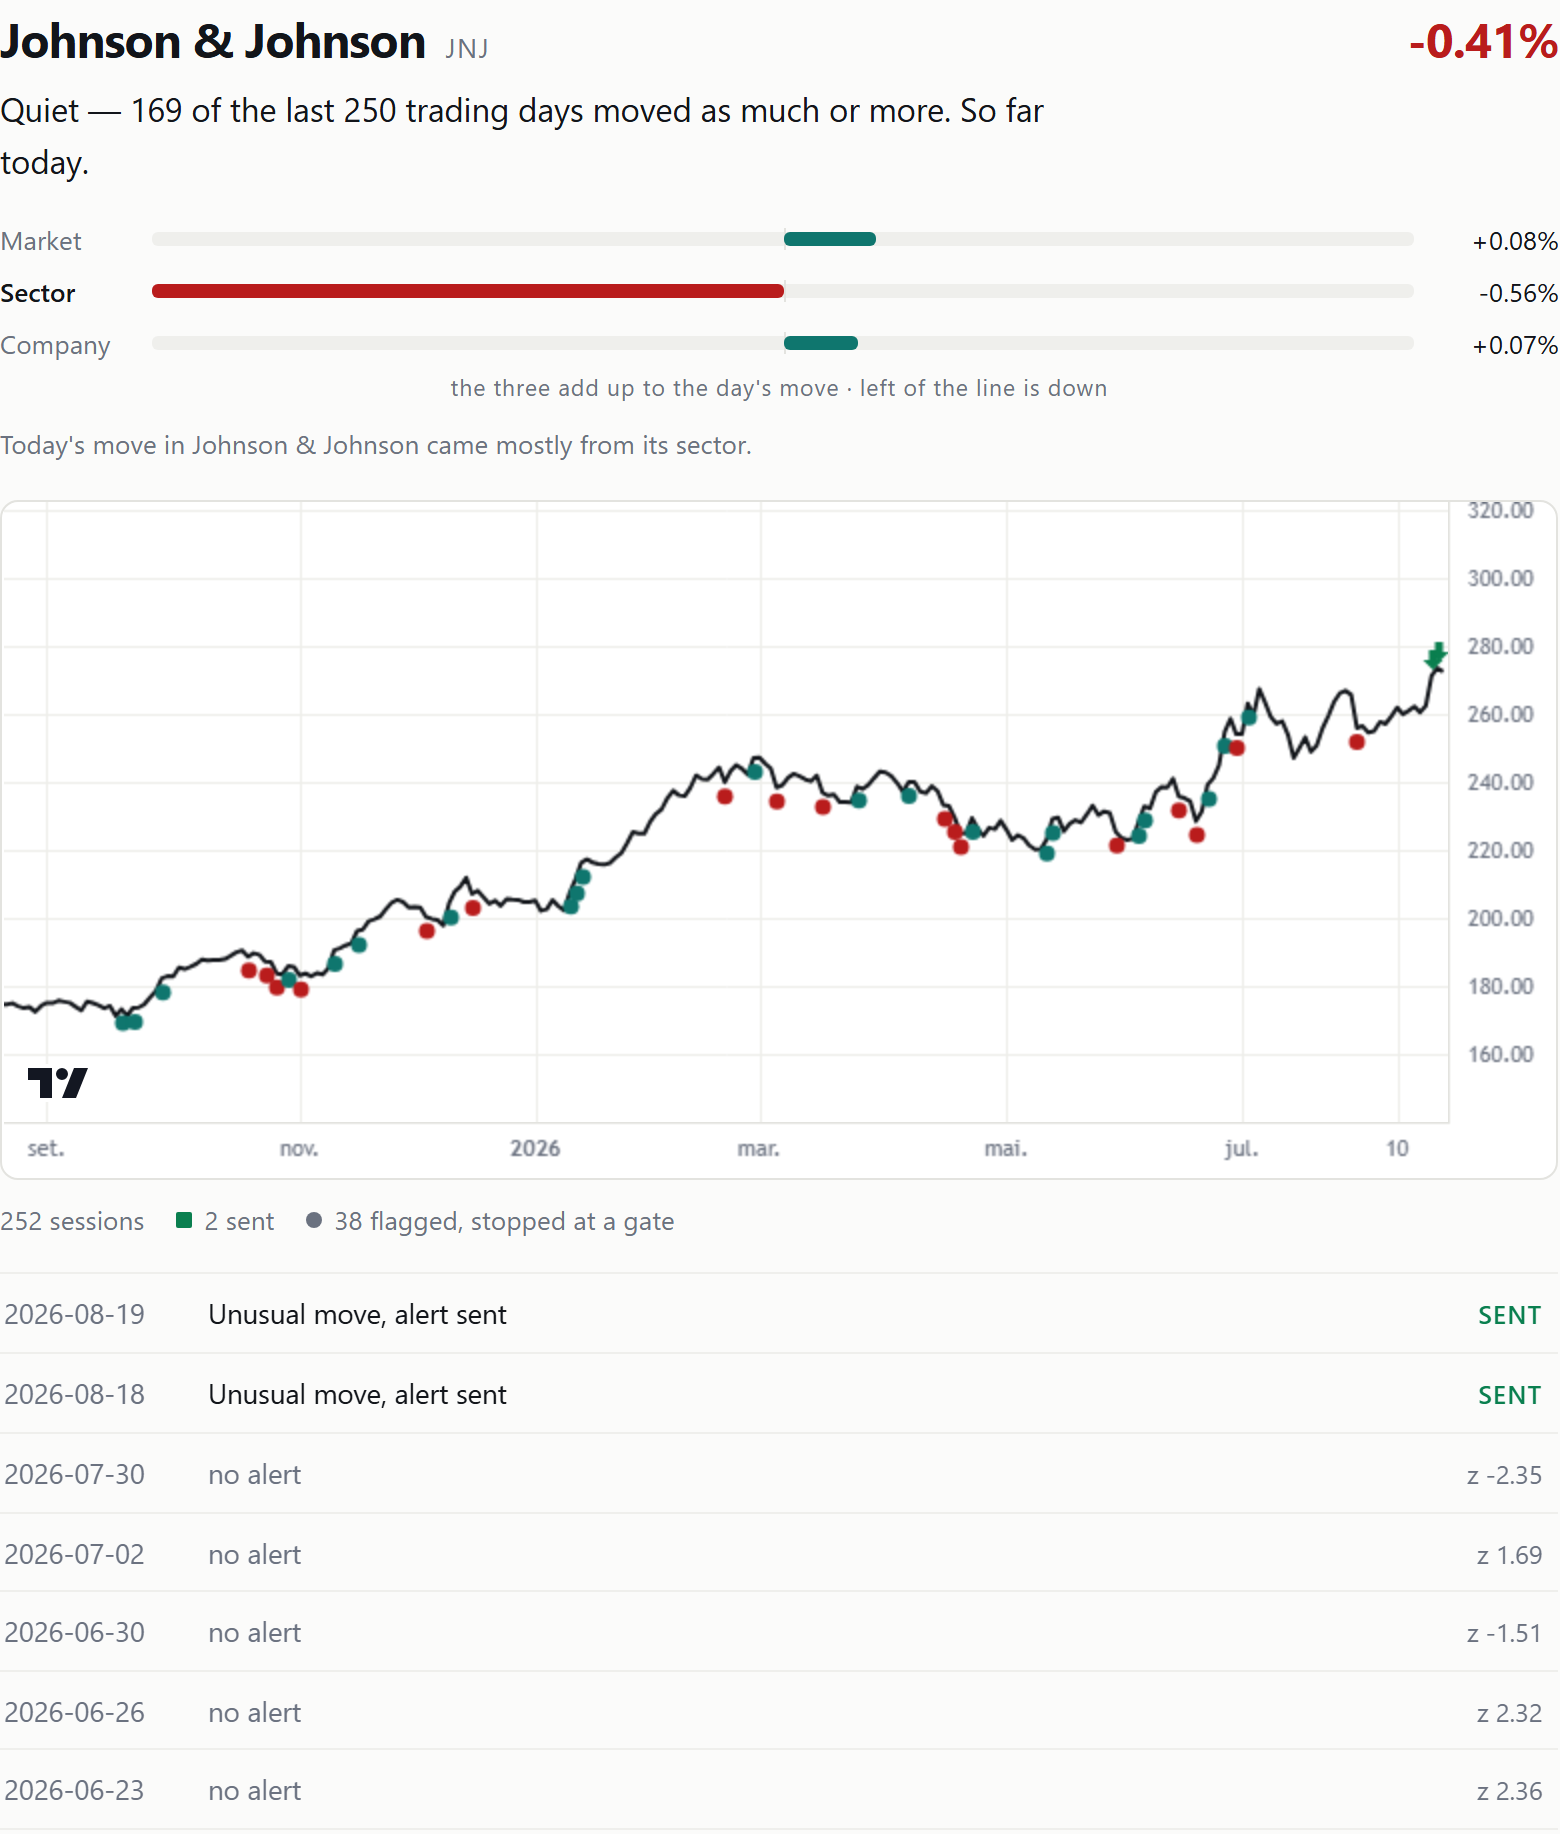
\includegraphics[width=\linewidth]{figures/app_v6_empresa.png}
\end{minipage}\hfill
\begin{minipage}[t]{0.50\textwidth}\centering

\includegraphics[width=\linewidth]{figures/app_v6_silencio.png}
\end{minipage}
\caption[Vistas da aplicação web]{Aplicação web em funcionamento a 20 de agosto de 2026, durante a
sessão norte-americana. À esquerda, a vista de uma empresa. À direita, as decisões do dia pela
ordem em que foram tomadas, com indicação da margem em falta quando aplicável.}
\label{fig:sis_pagina}
\end{figure}

A empresa apresentada na vista superior constitui um caso ilustrativo da segunda questão de
investigação, pela discordância entre a variação percentual e a repartição. A ação registava uma
descida de $0{,}41\%$; o mercado e a componente específica da empresa apresentavam valores
positivos, de $+0{,}08\%$ e $+0{,}07\%$; e a parcela que puxava o preço para baixo era a do setor,
com $-0{,}56\%$. A variação percentual isolada indica uma descida da empresa e conduz à procura de
uma causa interna que não existe. O veredicto termina na expressão \emph{``so far today''}, uma vez
que a captura corresponde a meio da sessão e não a um fecho.

\section{Implantação e operação}
\label{sec:sis_operacao}

O sistema corre como processo permanente, com ciclo de varredura de sessenta segundos, sobre
créditos de alojamento incluídos num plano académico. A primeira versão utilizava um agendador
gratuito de melhor esforço, cuja periodicidade efetiva era de aproximadamente hora e meia. A
alteração para processo permanente foi motivada pela redução do atraso dos alertas.

A latência foi medida sobre os $278$ alertas de notícia entregues entre 29 de julho e 30 de agosto
de 2026 que registam hora de publicação e hora de envio. A mediana do percurso completo é de $353$
minutos, com percentil noventa de $964$ minutos. A repartição localiza esse tempo sem ambiguidade:
a mediana entre a publicação e a deteção é de $353$ minutos, e a mediana entre a deteção e a
chegada da mensagem é de $5$ segundos, com percentil noventa de $16$ segundos. O sistema entrega em
segundos aquilo que a fonte lhe dá.

A separação por configuração não confirma a expectativa que motivou a alteração. Sobre os $28$
alertas entregues pelo agendador a mediana é de $196$ minutos; sobre os $250$ entregues pelo
processo permanente é de $402$ minutos. O ciclo mais curto não reduziu a latência observada. A
comparação não é interpretável como efeito do ciclo, uma vez que as duas configurações não
operaram em paralelo, entre elas alteraram-se as fontes de notícias e o período de calendário, e
as amostras são de dimensão muito desigual. O que a medição estabelece é que encurtar o ciclo só
compensaria se o tempo estivesse na cadência com que o sistema consulta a fonte, e não está.

Três causas concorrem para o atraso da descoberta, e este histórico não as separa. A primeira é a
fonte listar a notícia horas depois da hora que ela própria declara. A segunda é a notícia mais
recente do fluxo não ser a mais recente \emph{relevante}: numa amostra recolhida a 7 de agosto de
2026, o fluxo de uma das empresas trazia $250$ títulos com o mais recente publicado às 11:39, mas
o mais recente entre os $30$ relevantes era das 08:14. O alerta sai sobre o título correto, e é
esse título que é antigo. A terceira é o orçamento diário já estar gasto, que não aparece nesta
medição porque um alerta que não é entregue não regista hora de envio. Apenas a primeira seria
atenuada por um serviço pago de notícias, e a sua contribuição não está medida.

Todos estes valores constituem um limite inferior da latência sentida pelo utilizador, uma vez que
a hora de publicação é a declarada pela fonte e não o instante do acontecimento.

\subsection{Crescimento da base de casos}
\label{sec:sis_base}

Todo o título relevante observado pela varredura é conservado como candidato a precedente. Oito
dias depois, quando o impacto no preço se torna observável, o candidato é medido pela mesma regra
de alinhamento da Secção~\ref{sec:met_recuperacao} e integra a base de casos. O intervalo de
espera não constitui ineficiência: é a condição que impede um caso de conhecer o seu próprio
desfecho. A Figura~\ref{fig:sis_ciclo_kb} representa o ciclo.

\begin{figure}[ht]
\centering
\begin{tikzpicture}[font=\footnotesize, >={Stealth[length=2.2mm]},
  et/.style={draw, rounded corners=3pt, align=center, inner sep=4pt, text width=2.65cm,
             minimum height=1.25cm, fill=black!5},
  esp/.style={draw, dashed, rounded corners=3pt, align=center, inner sep=4pt, text width=2.4cm,
              minimum height=1.25cm, fill=white},
]
  \node[et]  (a) at (0,0)     {\textbf{dia $t$}\\ a varredura observa um título relevante};
  \node[esp] (b) at (3.55,0)  {conservado como candidato, com o seu vetor};
  \node[et]  (c) at (7.0,0)   {\textbf{dia $t+8$}\\ o impacto é observável};
  \node[et]  (d) at (10.5,0)  {integra a \textbf{base de casos}};

  \draw[->, thick, black!55] (a) -- (b);
  \draw[->, thick, black!55] (b) -- (c);
  \draw[->, thick, black!55] (c) -- (d);

  \draw[->, thick, black!55] (d.south) -- ++(0,-0.85) -| (a.south)
    node[pos=0.25, below, font=\scriptsize, black!65]
    {as avaliações seguintes comparam-se com os casos já maturados};
\end{tikzpicture}
\caption[Ciclo de crescimento da base de casos]{Percurso de um título entre a sua observação e a
sua disponibilidade como precedente. O intervalo de oito dias decorre de o impacto de um caso só
ser observável após o movimento do preço. O ciclo mantém atualizada a evidência apresentada pelo
sistema, e não os parâmetros do modelo: nenhum componente é retreinado.}
\label{fig:sis_ciclo_kb}
\end{figure}

O mecanismo atualiza a evidência exibida e não os parâmetros do modelo. Na taxonomia de deriva de
conceito de \textcite{gama2014survey}, o sistema dispõe da deteção da mudança e não da adaptação a
ela.

Verificou-se, com o sistema já em funcionamento, que este ciclo estivera interrompido durante
dezanove dias sem registo de qualquer erro. Os dois processos correm em máquinas separadas cujo
sistema de ficheiros é reinicializado a cada arranque, e os ficheiros intermédios de maturação não
estavam a ser publicados no repositório de dados. Corresponde à classe de custo que
\textcite{sculley2015debt} designam por dependência de dados não declarada: cada componente cumpre
o seu contrato, e a suposição que os liga não está expressa em parte alguma. O
Capítulo~\ref{cap:conclusoes} retoma o caso como limitação.

\section{Ciclo de vida do componente aprendido}
\label{sec:sis_ciclo}

O sistema treina um único modelo, que é a regressão logística de nove entradas descrita na
Secção~\ref{sec:met_triagem}. Medido contra uma linha de base de uma só variável, esse modelo
apresenta desempenho inferior, resultado reportado na Secção~\ref{sec:av_qi3}.

A contribuição de engenharia não reside na dimensão do modelo, mas na infraestrutura que torna
esse resultado, e a conclusão negativa que ele sustenta, defensáveis. Essa infraestrutura tem sete
componentes, cada um dos quais existe porque a sua ausência produziria um resultado favorável e
não verificável. A Figura~\ref{fig:sis_lifecycle} representa as duas metades do ciclo.

\begin{figure}[ht]
\centering
\begin{tikzpicture}[font=\scriptsize, >={Stealth[length=2mm]},
  cx/.style={draw, rounded corners=2pt, align=center, inner sep=3pt, text width=2.15cm,
             minimum height=1.0cm, fill=black!5},
  art/.style={cx, fill=black!14, draw=black!55, thick},
  obs/.style={cx, fill=white, draw=black!45},
  fase/.style={font=\scriptsize\bfseries, text=black!60},
]
  \node[fase] at (-1.55,0.95) {construção};
  \node[cx]  (d) at (0,0)    {conjunto de dados rotulado};
  \node[cx]  (t) at (2.5,0)  {treino};
  \node[cx]  (v) at (5.0,0)  {validação\\ \emph{calibração}};
  \node[cx]  (s) at (7.5,0)  {teste\\ \emph{utilização única}};
  \node[art] (m) at (10.0,0) {artefacto versionado};

  \foreach \xa/\xb in {d/t, t/v, v/s, s/m} \draw[->, thick, black!55] (\xa) -- (\xb);

  \node[fase] at (-1.55,-1.75) {observação};
  \node[art] (p) at (0,-1.9)   {o \textbf{mesmo} modelo, em produção};
  \node[obs] (g) at (2.5,-1.9) {registo de cada decisão};
  \node[obs] (w) at (5.0,-1.9) {espera pela resposta do preço};
  \node[obs] (r) at (7.5,-1.9) {pós-validação e deriva};

  \draw[->, thick, black!55] (m.south) -- ++(0,-0.5) -| (p.north);
  \foreach \xa/\xb in {p/g, g/w, w/r} \draw[->, thick, black!55] (\xa) -- (\xb);

  \draw[->, dashed, black!40] (r.east) -- ++(0.9,0) |- (10.0,-1.05)
    node[pos=0.72, right, align=left, text width=2.2cm, black!55]
    {retreino:\\ \textbf{ausente}};
\end{tikzpicture}
\caption[Ciclo de vida do componente aprendido]{As duas metades do ciclo. Na metade superior, a
construção: os dados são rotulados, a divisão é cronológica, a calibração é ajustada no bloco de
validação e o bloco de teste é utilizado uma única vez. Na metade inferior, a observação: o modelo
em produção é o modelo avaliado, cada decisão é registada, e dias mais tarde é confrontada com o
movimento efetivamente observado. A ligação a tracejado fecharia o ciclo e não existe: a deriva é
medida e não é corrigida.}
\label{fig:sis_lifecycle}
\end{figure}

\begin{description}
  \item[Construção do conjunto de dados.] O \gls{FNSPID} fornece títulos datados, e os preços
        provêm de fonte distinta. O alinhamento das duas séries, a atribuição de uma notícia de
        sábado ao dia de negociação correspondente, e a derivação do rótulo a partir do movimento
        futuro constituem o trabalho que produz os $79\,753$ exemplos da
        Secção~\ref{sec:met_dados}.

  \item[Declaração do rótulo como decisão.] A existência de movimento anormal nos três dias
        seguintes não é um facto presente nos dados: é uma definição, com limiar e horizonte
        escolhidos. A Secção~\ref{sec:av_qi3} mede nove definições alternativas em lugar de
        assumir a adotada.

  \item[Verificação da separação temporal.] Aos blocos cronológicos e ao embargo junta-se um
        teste executável: perturbado o futuro de um exemplo, as suas entradas têm de permanecer
        inalteradas e o seu rótulo tem de mudar. A ausência de fuga passa assim de afirmação a
        propriedade verificada a cada execução.

  \item[Calibração com enviesamento medido.] A saída do classificador é um valor no intervalo
        unitário, que serve simultaneamente para ordenar candidatas e para as excluir. O ajuste de
        Platt corre sobre um bloco que nunca participou no treino, e a discrepância de prevalência
        entre esse bloco e o de teste é declarada no Capítulo~\ref{cap:avaliacao} em vez de ficar
        implícita.

  \item[Versionamento dos artefactos.] O modelo treinado, o calibrador e um descritor da execução,
        contendo dimensão de cada bloco, prevalência, semente e métricas, residem no repositório.
        Uma métrica desacompanhada do artefacto que a produziu não é reproduzível.

  \item[Identidade entre modelo avaliado e modelo implantado.] O codificador de frases utilizado
        na avaliação depende de uma biblioteca cujo volume excede o contentor de produção. Em vez
        da substituição por outro modelo, que faria a dissertação descrever um sistema distinto do
        que se encontra em funcionamento, o mesmo modelo foi exportado para formato de execução
        leve e a fidelidade da conversão foi medida.

  \item[Observação do sistema implantado.] Cada decisão de triagem é registada. Decorridos os dias
        necessários, um segundo procedimento rotula essas decisões pela mesma regra utilizada no
        treino e mede o contributo do modelo. Foi por esta via que se estabeleceu a ausência de
        contributo reportada na Secção~\ref{sec:av_qi3}. A deriva das entradas é medida pelo mesmo
        mecanismo.
\end{description}

\subsection{Componentes desenvolvidos e componentes consumidos}

O único modelo consumido do exterior é um codificador de frases pré-treinado, utilizado sem
qualquer ajuste. O trabalho não reivindica contribuição sobre esse componente além da sua seleção
por medição, efetuada contra quatro alternativas, entre as quais um modelo de maior dimensão, dois
codificadores mais recentes e um modelo específico do domínio financeiro, que apresentou o pior
desempenho do conjunto. A dependência é essencial, uma vez que não existe recuperação semântica
sem representação de frases, e é simultaneamente substituível: a interface que o isola dispõe de
uma implementação alternativa que degrada para sobreposição lexical quando o modelo não está
disponível.

Foi desenvolvido no âmbito deste trabalho tudo o resto. O conjunto de dados rotulado e o
procedimento de alinhamento que o protege de fuga temporal. O detetor, com a janela de estimação
que exclui o dia explicado. A repartição do movimento com encolhimento dos coeficientes. A base de
precedentes com impacto medido. O classificador de triagem e a sua calibração. A política de
decisão e as constantes da Tabela~\ref{tab:sis_portas}. A camada que compõe o texto a partir dos
objetos calculados. E o mecanismo que observa o sistema depois de implantado.

O sistema não integra um modelo de linguagem na produção do texto entregue ao utilizador. A
ausência é deliberada e decorre do argumento desenvolvido na Secção~\ref{sec:ctx_xai}: uma frase
gerada constitui uma afirmação, ao passo que o sistema descrito entrega afirmações acompanhadas da
evidência que as sustenta.

\subsection{O elo em falta: arquitetura de retreino}

O ciclo não inclui retreino. Os parâmetros correspondem ao período de 2018 a 2023 e não foram
reajustados, apesar de a deriva se encontrar medida e de o índice de estabilidade populacional
situar a entrada principal na banda de deslocamento significativo. A operação seria tecnicamente
possível, dado que os rótulos novos derivam dos preços observados; o impedimento é que o retreino
com o registo de produção alteraria os valores reportados neste documento, e a avaliação dessa
alteração exige tempo de observação que não estava disponível.

A ausência de execução não dispensa, contudo, a definição da arquitetura. A
Figura~\ref{fig:sis_retreino} apresenta o ciclo de treino contínuo desenhado para este sistema, com
os mecanismos que o tornariam seguro. Três decisões o caracterizam.

A primeira é o \textbf{gatilho}, condicional e não temporal. O retreino desencadeia-se quando o
índice de estabilidade populacional de qualquer entrada ultrapassa $0{,}25$, o limiar convencional
de deslocamento significativo, ou ao fim de três meses sem revisão. A segunda é a \textbf{janela
deslizante}: o treino cobre os vinte e quatro meses anteriores ao gatilho, e a validação e o teste
os períodos seguintes, com o embargo de cinco dias da Secção~\ref{sec:met_triagem}. A divisão
permanece cronológica, porque o problema não deixa de ser temporal por o modelo ser novo.

A terceira, e a que distingue um ciclo de treino contínuo de uma automatização perigosa, é a
\textbf{porta de promoção}. Um modelo recém-treinado não substitui o modelo em vigor por ser mais
recente: substitui-o apenas se o superar sobre o mesmo bloco de teste reservado, e se a
sobreposição do intervalo de confiança da diferença excluir zero. Um modelo que não passe essa
porta é registado e descartado, e o modelo em vigor permanece com a deriva declarada. É a diferença
entre adaptar-se à mudança e perseguir ruído.

\begin{figure}[ht]
\centering
\begin{tikzpicture}[font=\scriptsize, >={Stealth[length=2mm]},
  cx/.style={draw, rounded corners=2pt, align=center, inner sep=3pt, text width=2.35cm,
             minimum height=0.95cm, fill=black!5},
  gat/.style={cx, dashed, fill=black!12},
  art/.style={cx, fill=black!16, draw=black!55, thick},
]
  \node[cx]  (p) at (0,0)     {registo de decisões em produção};
  \node[cx]  (m) at (2.9,0)   {maturação:\\ 8 dias};
  \node[cx]  (r) at (5.8,0)   {rótulos novos, da mesma regra};
  \node[gat] (g) at (8.7,0)   {\textbf{gatilho}\\ PSI $>0{,}25$\\ ou 3 meses};
  \node[cx]  (t) at (8.7,-1.9) {retreino em janela de 24 meses};
  \node[cx]  (v) at (5.8,-1.9) {validação e calibração novas};
  \node[gat] (q) at (2.9,-1.9) {\textbf{porta de promoção}\\ supera o em vigor?};
  \node[art] (n) at (0,-1.9)   {promove\\ e versiona};

  \foreach \a/\b in {p/m, m/r, r/g} \draw[->, thick, black!55] (\a) -- (\b);
  \draw[->, thick, black!55] (g) -- (t);
  \foreach \a/\b in {t/v, v/q, q/n} \draw[->, thick, black!55] (\a) -- (\b);
  \draw[->, thick, black!55] (n.north) |- ++(0,0.75) -| (p.south);
  \draw[->, dashed, black!45] (q.north) -- ++(0,0.72)
    node[above, align=center, black!60] {não supera:\\ regista e descarta};
\end{tikzpicture}
\caption[Arquitetura de retreino desenhada e não executada]{Ciclo de treino contínuo definido para
este sistema e não executado no âmbito deste trabalho. O gatilho é condicional e não temporal; a
janela é deslizante e a divisão permanece cronológica com embargo; e a porta de promoção impede que
um modelo novo substitua o modelo em vigor sem o superar sobre um bloco reservado. A ligação a
tracejado é o caminho de rejeição, e a sua existência é o que distingue o ciclo de uma
automatização que persegue ruído.}
\label{fig:sis_retreino}
\end{figure}

O ciclo não inclui igualmente qualquer forma de verdade humana. Os três rótulos utilizados neste
trabalho, correspondentes a movimento anormal, pertença ao mesmo setor e percentil de movimento,
constituem aproximações verificáveis que nunca foram confrontadas com o julgamento de um
avaliador humano. É a limitação de que as restantes mais dependem, e o
Capítulo~\ref{cap:conclusoes} retoma-a.
